\section{System Behavior}
\label{section:sysBehavior}

The use case view is the prime motivator for the System Behavior.
This is because the program is simple with no complex components.

The program starts with the triangle filled in, demonstrated by the left triangle in Figure \ref{Fig:Fig1}, and then progresses onward infinitely until the Escape Key is pressed.
The code describing this behavior will be explained further in Section \ref{section:logView}.

\begin{figure}[htb]
    \centering
    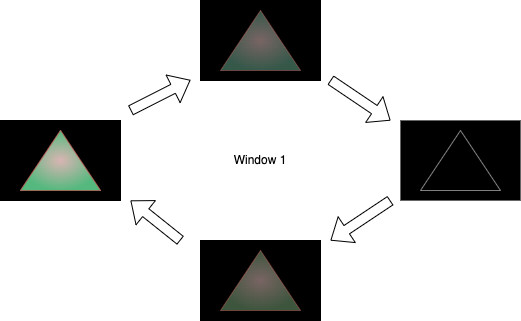
\includegraphics[width=10cm]{./Images/SysBehavior.png}
       \caption{System Behavior for Window 1.}
           \label{Fig:Fig1}
\end{figure}

In Figure \ref{Fig:Fig1}, the right triangle has a white outline and black fill to demonstrate that the triangle exists, but lacks color.
When the program is run however, the triangle loses color until it is not visible anymore.